\documentclass[a4paper, 10pt]{article}
\usepackage{graphicx, float, url, hyperref, lscape, afterpage, amsthm, amsmath, amsfonts, booktabs}
\usepackage[margin=1in]{geometry}
\title{Stochastic Storm Surge Modeling in the Philippine Archipelago using ADCIRC+SWAN through Parallel Computing}
\author{CS 294 Final Report\\\\ Joshua Frankie Rayo\\ Scientific Computing Laboratory}
\date{\today}
\newtheorem{definition}{Definition}
\newtheorem{theorem}{Theorem}
\newtheorem{assumption}{Assumption}

\begin{document}
	\maketitle
	
	\begin{abstract}
		There is a strong need to model and simulate stochastic storm surges for it to be more realistic. But until today there is still no CFD model that does this. In this paper, we will propose a methodology that allows to incorporate stochastic process in the fluid momentum equations to finally simulate stochastic storm surge. The objective of this research is to modify the 3D Advanced Circulation (ADCIRC) Model to include stochastic process in the governing equations. A random term will be added to the 3D momentum equations that solves the velocity of a fluid. Additive noise will be considered together with Gaussian process. We will particularly simulate the storm surge phenomena happened in Tacloban City during the landfall of typhoon Haiyan on November 05, 2013 and compare its results.
	\end{abstract}
	
%	\tableofcontents
%	\listoffigures
%	\listoftables
	
	\section{Introduction}
	Philippines is a typhoon-prone country in Southeast Asia. About 20 typhoons affect our country every year.
	
	Typhoon Haiyan that made landfall at Eastern Samar in November 8, 2013 brought destructive storm surge. Haiyan developed into a Category 5 typhoon with wind speeds of 250 km/h that caused storm surge to elevate up to 5 meters. It brought devastating effects particularly in Tacloban City. More than 6,000 people are confirmed dead and 1.14 million houses damaged. Overall economic losses are estimated at 571.1 billion Pesos.
	
	On top of that, surge height predictions from different agencies are not completely consistent. The JRC data indicate a storm surge South of the eye while Deltares sees this at the North of the typhoon. Deltares indicated maximum water height of 5 meters while JRC indicated about 2.3 meters. Project NOAH published its own data and indicated maximum water height of 5.16 meters. Thus, the country demands for a better and more realistic storm surge modeling.
	
	When water enters the shore, the model should also account for random forces exerted by certain debris. This calls for a storm surge model that includes random external force as a stochastic process in the governing equations. However, there is still no CFD software that does this.
	
	\section{Research Objective}
	The research aims to tailor a model specifically for the Philippines and designing it to compute fast enough and give real-time storm surge predictions around the country.
	To incorporate external forcing by random debris like rocks and structural materials, we will modify the numerical formulation of an existing model and hopefully give more realistic storm surge simulations.
	We will be using ADCIRC+SWAN model \cite{bib:adcirc} for this research.
	
	\section{Review of Related Studies}
	\subsection{Storm Surge Modeling}
	Storm surge simulation can be done using deterministic models or statistical analysis from historical data. As of today, there are no CFD software or package that solves stochastic Navier-Stoles equations for storm surge that accounts for random forcing. Two popular deterministic 3D models exist, namely ADCIRC+SWAN and Delft3D-FLOW+WAVE. Detailed comparison of these models is given below:
	
	\begin{table}[H]
		\begin{tabular}{l|ll}
			\textbf{Feature} & \textbf{ADCIRC+SWAN} & \textbf{Delft3D-FLOW+WAVE} \\
			\hline
			Governing equations & 3D shallow water eqn & 3D shallow water eqn\\
			Spatial discretization & finite-element & curvilinear grid\\
			$\sigma$-coordinate system & yes & yes\\
			Parallel computation & yes & no\\
			Tidal forcing & yes & yes\\
			Meteorological forcing & yes & yes\\
			Wave modeling & yes & yes\\
			License & open-source & open-source\\
		\end{tabular}
		\caption{Comparison of features between ADCIRC and Delft3D}
	\end{table}
	Other models like SLOSH and JMA are disregarded, as their governing equations are only in 2D we want to settle with better models.
	
	\subsection{Why ADCIRC+SWAN?}
	Aside from the comparison given above, ADCIRC+SWAN employs mass and momentum conservation as well as grid flexibility. Nonlinear terms are retained in its equations. It has also been optimized for enhanced performance on parallel computers; its efficiency and accuracy is well-understood and documented due to extensive numerical analysis of the source codes \cite{bib:adcirc}. Its ability to compute in parallel is a great factor in considering this model since our objective is to provide real-time storm surge predictions.
	
	\section{Governing Equations of 3D ADCIRC+SWAN}
	ADCIRC uses the shallow water form of the momentum equations, applying the Boussinesq and hydrostatic pressure approximations \cite{bib:num}. 
	The equations are identical to their Cartesian counterparts except that $\partial/\partial x$ terms are multiplied by the spherical coordinate correction factor, $S_p$ \cite{bib:num}. The horizontal momentum equations are given by the following equations:
	
	\begin{align*}
	\frac{\partial u}{\partial t} + u S_p \frac{\partial u}{\partial x} + v \frac{\partial u}{\partial y} + w \frac{\partial u}{\partial z} - fv = -g S_p \frac{\partial \left[\zeta + p_s/g \rho_0 - \alpha \eta\right]}{\partial x} + \frac{\partial}{\partial z} \left(\frac{\tau_{zx}}{\rho_0}\right) - b_x + m_x \\
	\frac{\partial v}{\partial t} + u S_p \frac{\partial v}{\partial x} + v \frac{\partial v}{\partial y} + w \frac{\partial v}{\partial z} + fu = -g \frac{\partial \left[\zeta + p_s/g \rho_0 - \alpha \eta\right]}{\partial y} + \frac{\partial}{\partial z} \left(\frac{\tau_{zy}}{\rho_0}\right) - b_y + m_y
	\label{eqn:sph}
	\end{align*}
	
	Coupled with the continuity equation to solve for the vertical velocity
	\begin{equation*}
	\nabla \cdot \vec{u} = S_p \frac{\partial u}{\partial x} + \frac{\partial v}{\partial y} + \frac{\partial w}{\partial z} = 0
	\end{equation*}
	
	where
	\begin{itemize}
		\item $\langle u, v, w \rangle$, velocity components
		\item $p(x, y, z, t)$, pressure scalar field
		\item $\rho(x, y, z, t)$, fluid density
		\item $u/v/w(x, y, z, t)$, velocities in the $x$, $y$, and $z$ directions
	\end{itemize}
	
	Consequently, these equations comprise a generalized set of equations that allows ADCIRC to function using either a Cartesian horizontal grid (by setting $S_p = 1$) or in spherical grid \cite{bib:num} is a very efficient manner.
	
	\subsection{Numerical Formulation of ADCIRC}
	In the numerical formulation of ADCIRC, variational formulation was applied twice: multiply each term by a horizontal weighting function $\phi_j$ and integrate on the horizontal domain, then multiply the result by a vertical weighing function $\psi_k$ and integrate over the vertical domain \cite{bib:num}. After applying Galerkin finite-element method, the equation above reduces to the form of the 3D momentum equations solved in ADCIRC. The equation reduces to a tridiagonal matrix structure $\mathbf{Mq = F}$ and this is solved by Jacobi conjugate gradient method \cite{bib:num}. Noise can be added to the force vector $\mathbf{F}$.
	
	\subsection{Parameter Sensitivity}
	There is already a study \cite{bib:wetdry} regarding the parameter sensitivity of ADCIRC+SWAN by R. A. Luettich, Jr., et. al. and we are just validating their findings.
	\subsubsection{Wetting and Drying Algorithm}
	ADCIRC+SWAN also included wetting and drying algorithm to simulate wetting and drying of nodes described by the following:
	\begin{enumerate}
		\item If the water total depth is larger than $H_{min}$ (water cutoff depth), the node remains "wet" and included in the rest of calculations.
		\item Else, the node is "dry" and removed from the calculations.
		\item If the minimum wetting velocity is larger then $U_{min}$, the node becomes "wet".
	\end{enumerate}
	\begin{equation*}
	U = \frac{g\left(\zeta_{i-1} - \zeta_i\right)}{\tau_i \Delta x_i}
	\end{equation*}
	This criterion almost becomes a height restriction if the adj node's free surface circulation is sufficiently larger than its own. In the previous study, $U_{min}$ does not have a significant effect regarding sensitivity, so we do not include this in our analysis.
	
	\subsubsection{Bottom Friction Coefficient}
	Denoted by $\tau_0$, this controls the bottom friction coefficient in the momentum equations. Then the bottom friction for each node $i$ is given by
	\begin{equation*}
	\tau_i = \tau_0 \left(\frac{u_i}{H_i}\right)
	\end{equation*}
	Note that $\tau \propto \tau_0$ and $\tau_i$ increases in shallower, near-shore waters and directly affects the speed at which waves inundate or recede.
	
	\subsubsection{GWCE Weighing Factor}
	The parameter $G$ is the numerical parameter that controls the balance between the wave continuity equation and the primitive continuity equation.
	\begin{equation*}
	\frac{\partial \zeta}{\partial t} + G\zeta - \nabla \cdot M = 0
	\end{equation*}
	Note that as $G \rightarrow 0$ it is a pure wave equation, $G \rightarrow \infty$ it is a pure primitive equation. If $G$ is set too high the solution has spurious oscillations and prevent the model from capturing the behavior of waves.
	
	\section{Methodology}
	Gaussian noise will be added to the right side of the equation to simulate random forcing and the module \texttt{timestep.f} will be modified. Notice that it is only the finite-element formulation of the momentum equation will be modified. Additive noise starts at $0$ then subsequent values are to be governed by OU process. Additive noise signifies that there are random forces that are exerted by some debris, and colored noise are more evident in nature than white noise.
	
	Sensitivity of some parameters mentioned above will also be analyzed including minimum height, weighing factor of generalized wave continuity equation, bottom friction coefficient and variance of the noise. Each parameter will be analyzed keeping other parameters in their default values to know the significance of each.
	
	Surface elevation will be measured on three points in the domain: near Tacloban airport, near Tacloban main and an outstanding location.
	
	\begin{figure}[H]
		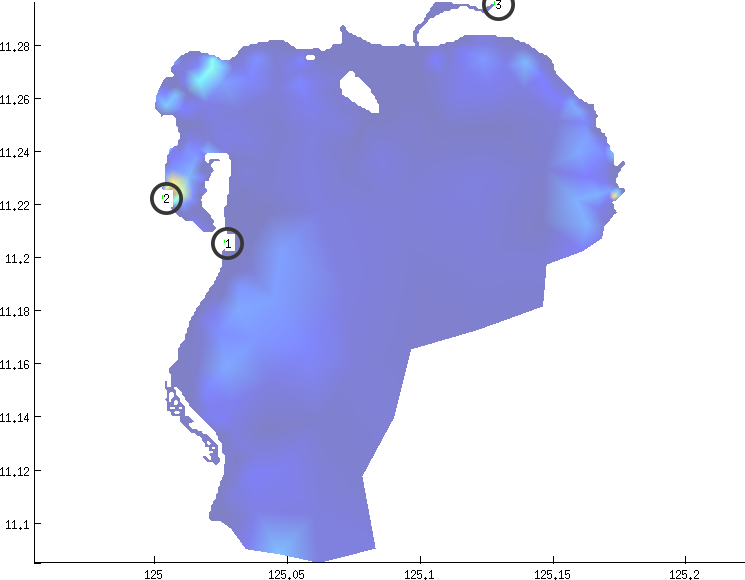
\includegraphics[width=.5\textwidth]{stations}
	\end{figure}
	
	\section{Preliminary Results}
	\subsection{Surge Simulation, Deterministic Case}
	The figure below shows the time-series water elevation on three observation points:
	
	\begin{figure}[H]
		
\includegraphics[width=.5\textwidth]{stoch0}
		
\includegraphics[width=.5\textwidth]{stoch0snap}
	\end{figure}
	
	Based on the simulation, peak surge height is 5.37 meters around 6pm of November 08, 2013 near Tacloban airport while negative surges happened on the other side of Tacloban Bay, suggesting conservation of mass.
	
	\subsection{Stochastic Case}
	Gaussian noise is added to the force vector in the module \texttt{timestep.f} with zero mean and variance of $\sigma = 10^{-3}$. From the uniform random number generator inherent in Fortran, it is possible to generate normal random numbers using the technique called ratio of uniforms augmented with quadratic bounding curves by A.J. Kinderman and J.F. Monahan. The figure below shows the effect (a realization) of additive noise on water elevation on three stations:
	
	\begin{figure}[H]
		
\includegraphics[width=.5\textwidth]{stochn1}
		
\includegraphics[width=.5\textwidth]{stochn1snap}
	\end{figure}
	
	Peak surge height was 5.34 meters compared to 5.37 meters from the original. Since we only added noise with very small variance, there is little difference in the results compared to the deterministic case. As we observe, the curves are still smooth because of the predictor-corrector algorithm employed by the model on its numerical formulation. We also observed that the model is very sensitive to noise and stronger noise lead to unstable computation. Despite noise, surface elevation contours still show coherent structures.
	
	\subsection{Sensitivity Analysis}
	Back to the deterministic model, some of the parameters that are modified in the model parameter file are set to the following default values
	\begin{itemize}
		\item $H_{min} = 0.10$
		\item $\tau_0 = 0.15$
		\item $G = 0.01$
	\end{itemize}
	and produced the following time-series surface elevation on three stations, figure below:
	
	\begin{figure}[H]
		
\includegraphics[width=\textwidth]{stoch0}
	\end{figure}
	
	Results are three days from November 07, 2013, the date before Haiyan made landfall. Height ($y$-axis) is in meters and time ($x$-axis) is in days. Peak surge height occured on November 08, 2013 before 6 pm predicted at 5.36 meters.
	
	\subsubsection{Water Cutoff Depth}
	The figures below represent time-series graphs of surface elevation as $H_{min}$ parameter is varied. Values are: 0.01, 0.05, 0.10, 0.15, 0.20, 0.25, 0.3 and 0.4. Figures are to be read from left to right and top to bottom.
	
	\begin{figure}[H]
		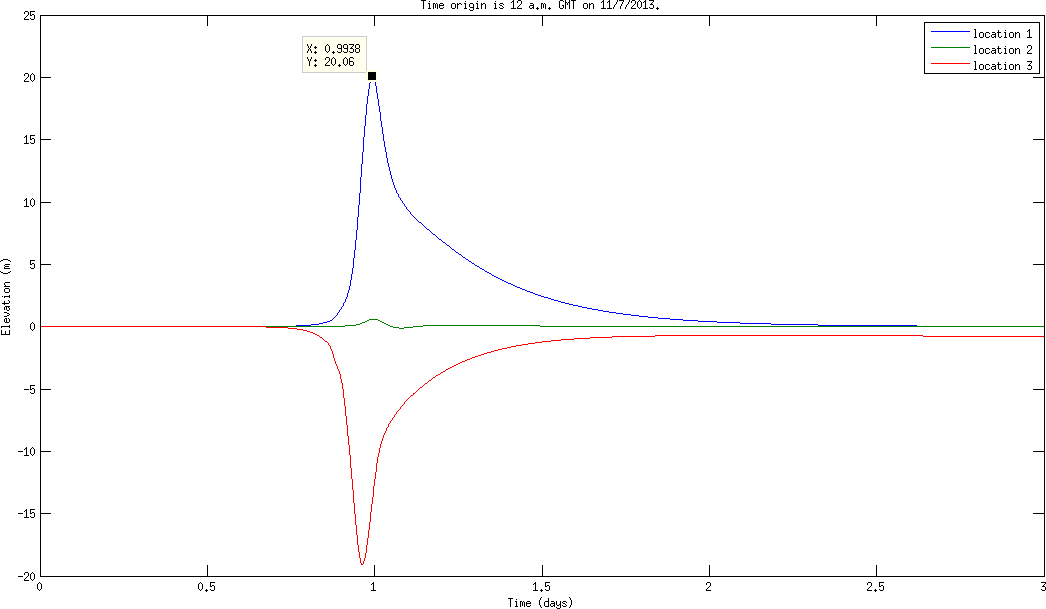
\includegraphics[width=.5\textwidth]{H_min/h0-01}	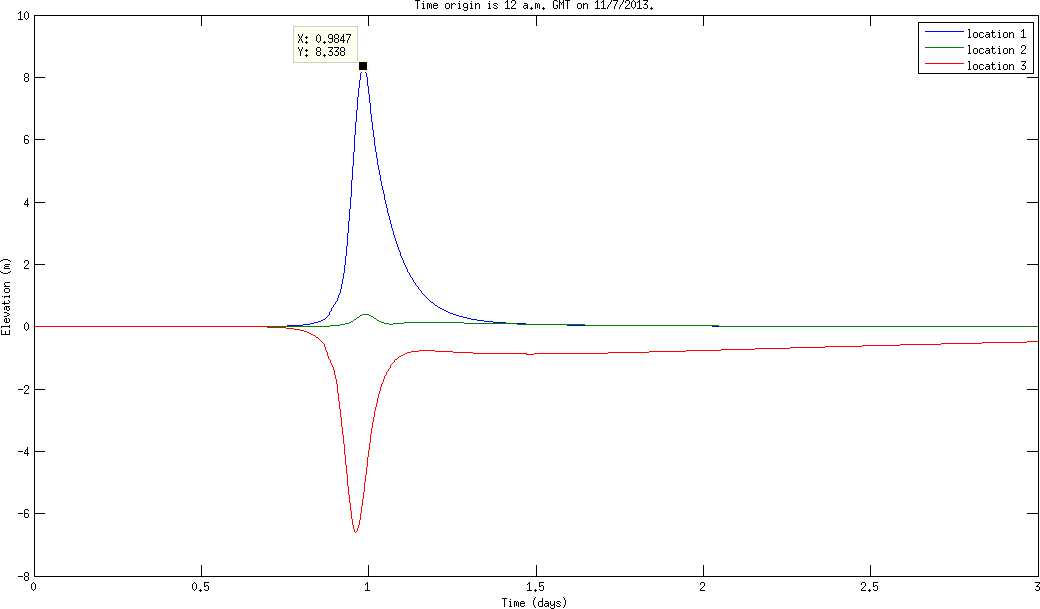
\includegraphics[width=.5\textwidth]{H_min/h0-05}
		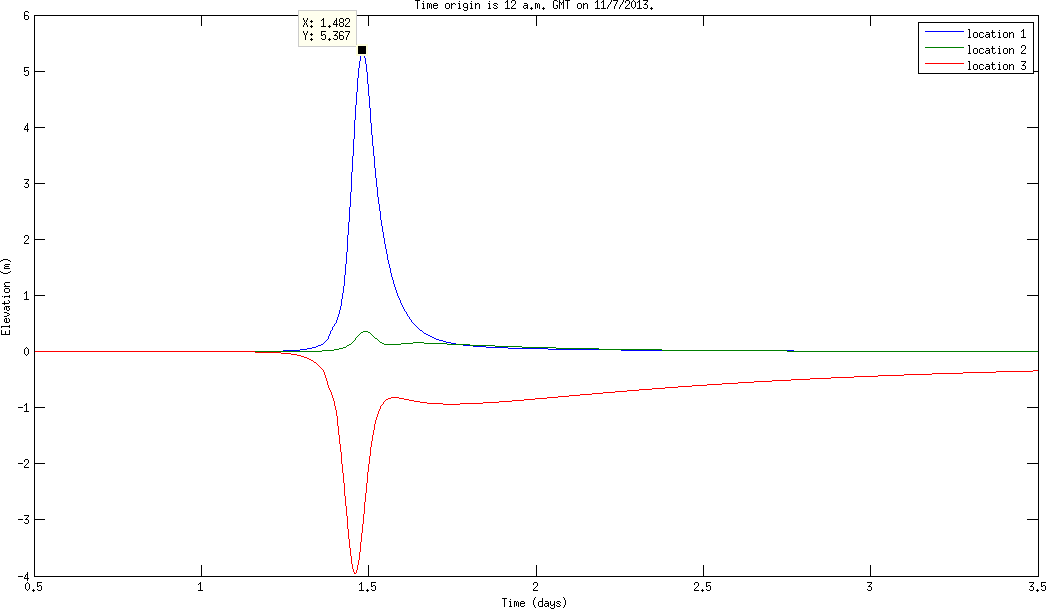
\includegraphics[width=.5\textwidth]{H_min/h0-1}
		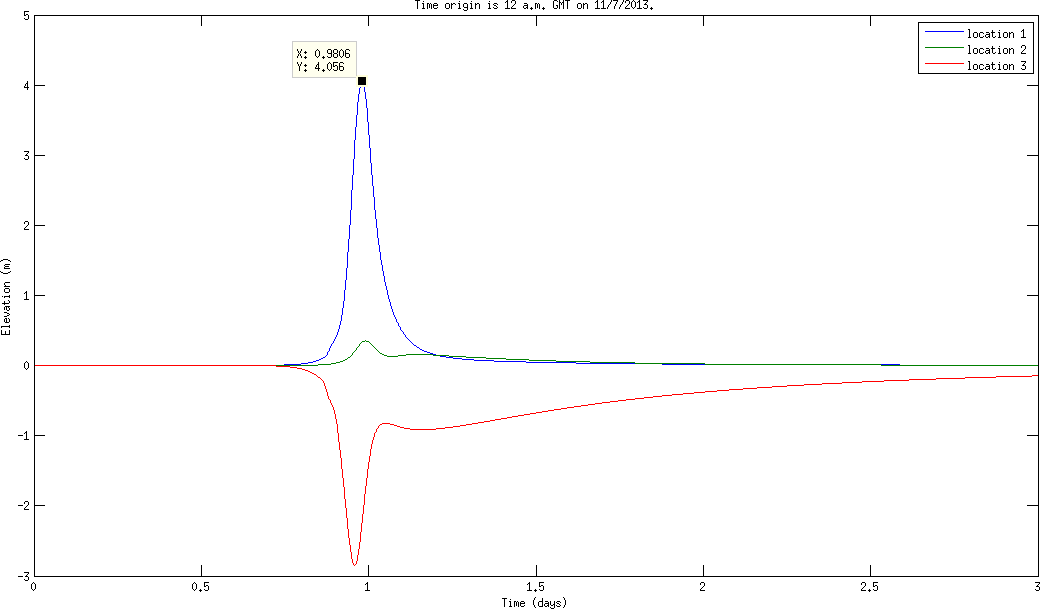
\includegraphics[width=.5\textwidth]{H_min/h0-15}
	\end{figure}
	\begin{figure}[H]
		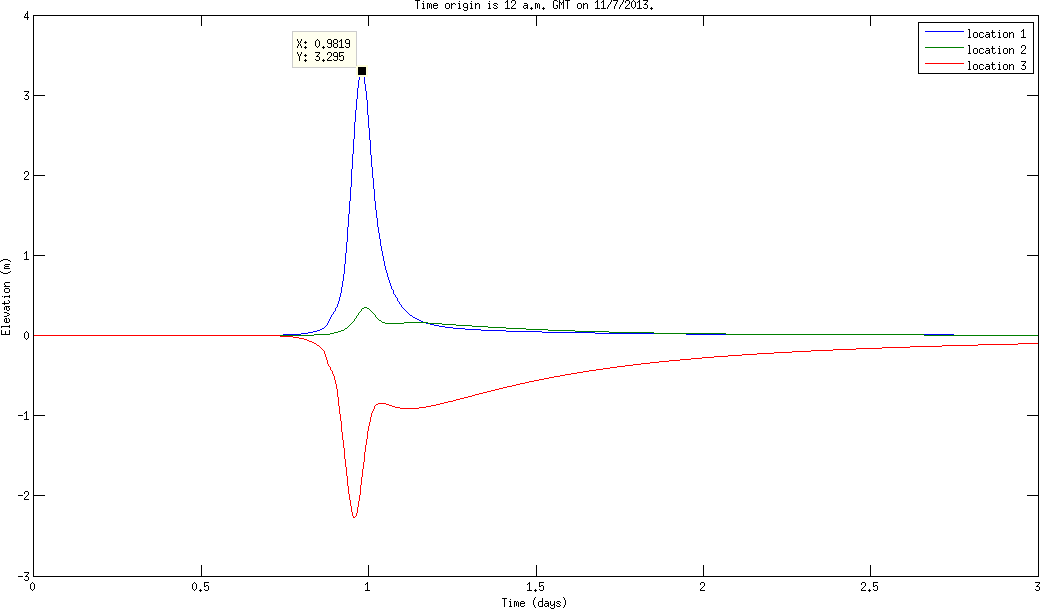
\includegraphics[width=.5\textwidth]{H_min/h0-2}
		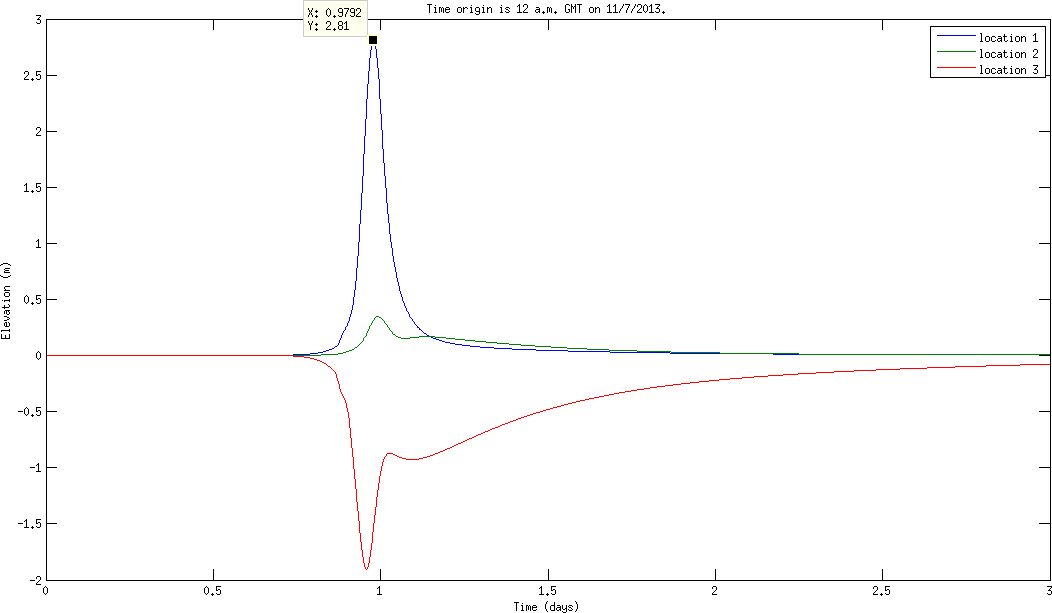
\includegraphics[width=.5\textwidth]{H_min/h0-25}
		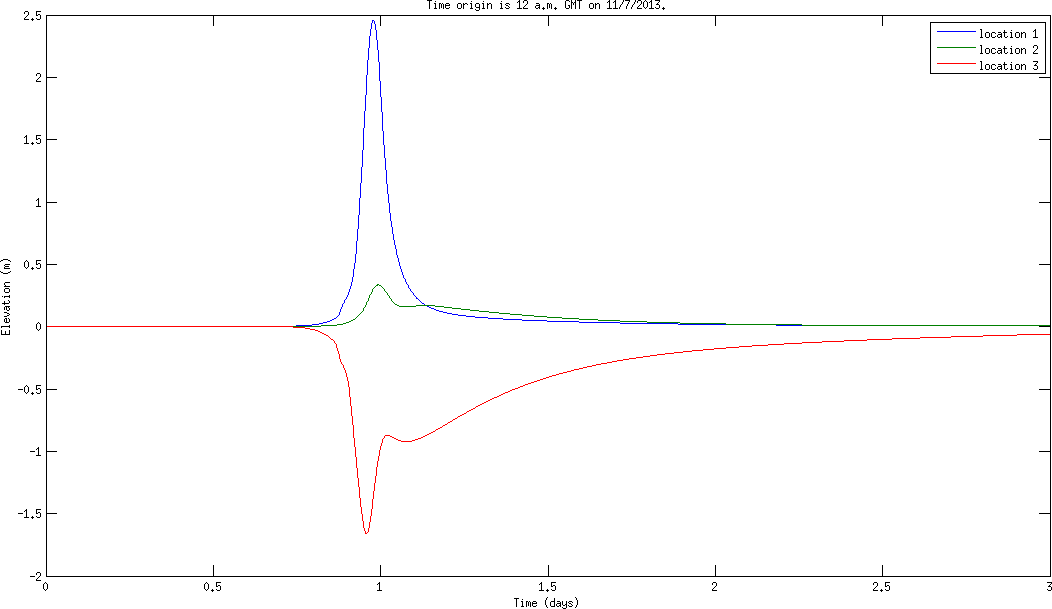
\includegraphics[width=.5\textwidth]{H_min/h0-3}
		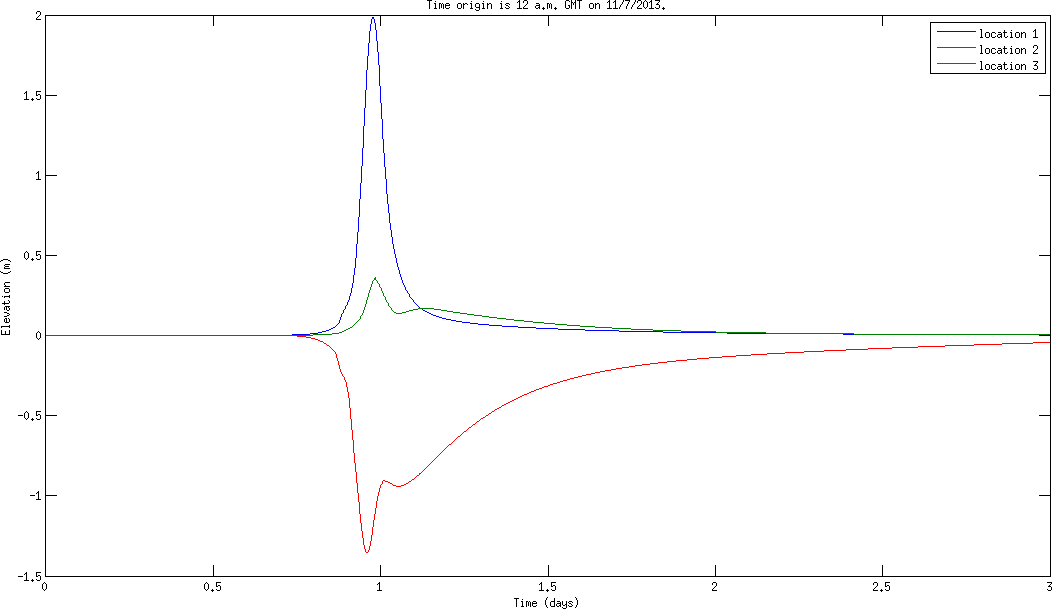
\includegraphics[width=.5\textwidth]{H_min/h0-4}
	\end{figure}
	
	As $H_{min}$ becomes smaller, peak surface elevation becomes higher. Peak surge height ranges from 2 meters up to 20 meters by tweaking this parameter.
	
	\subsubsection{Bottom Friction Coefficient}
	The figures below represent time-series graphs of surface elevation as $\tau$ parameter is varied. Values are: 0.01, 0.05, 0.10 and 0.20. Figures are to be read from left to right and top to bottom.
	
	\begin{figure}[H]
		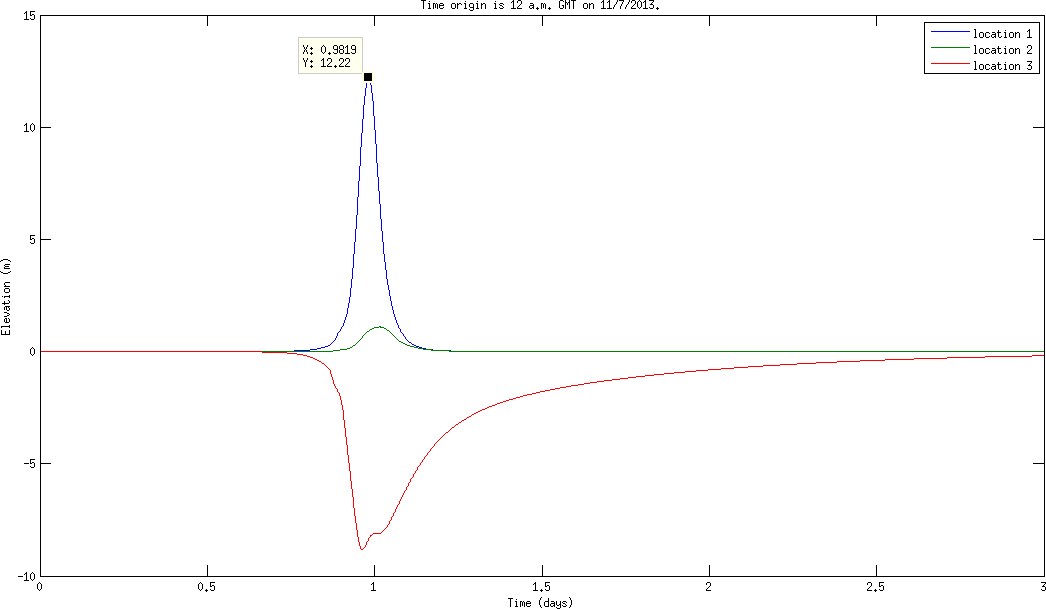
\includegraphics[width=.5\textwidth]{Tau/tau0-01}
		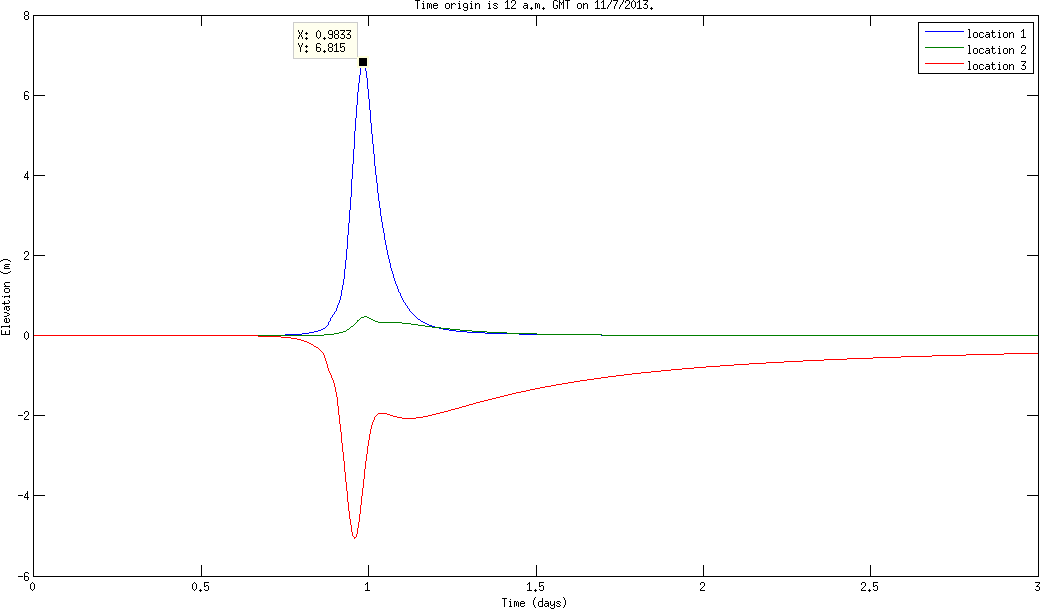
\includegraphics[width=.5\textwidth]{Tau/tau0-05}	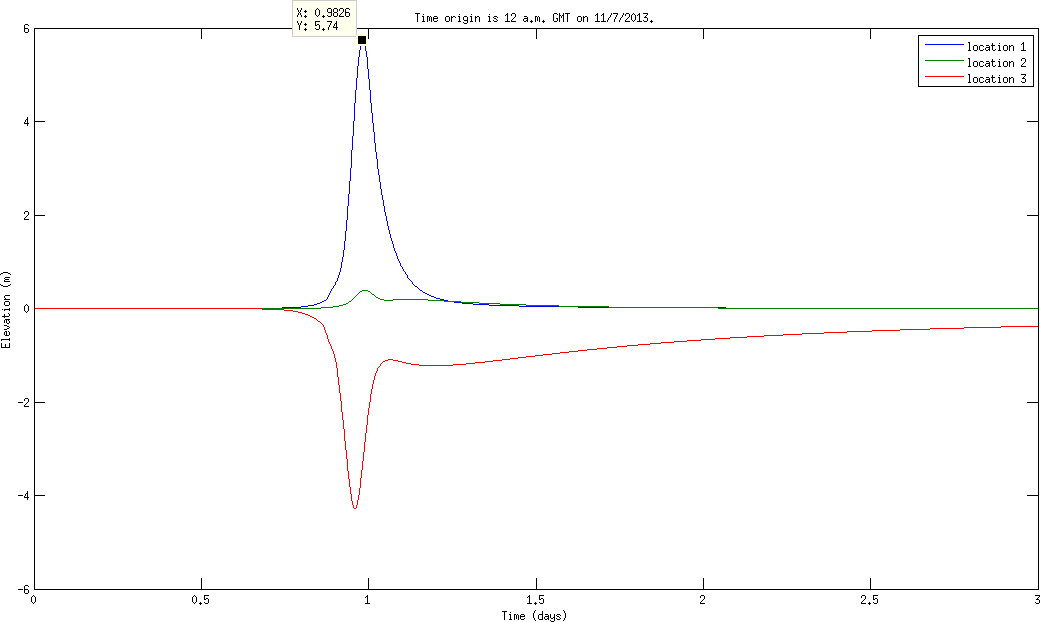
\includegraphics[width=.5\textwidth]{Tau/tau0-10}
		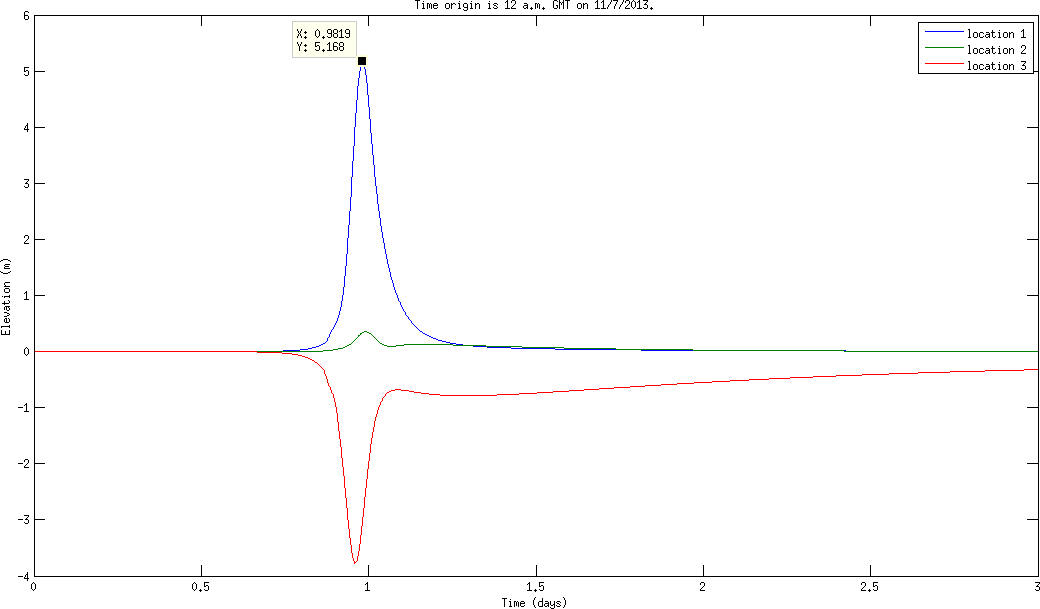
\includegraphics[width=.5\textwidth]{Tau/tau0-20}
	\end{figure}
	
	As $\tau$ becomes smaller, peak surface elevation becomes higher and water subside slower, as also described in the related study. Peak surge height ranges from 2 meters up to 20 meters.
	
	\subsubsection{GWCE Weighing Factor}
	The figures below represent time-series graphs of surface elevation as $G$ parameter is varied. Values are: 0.001, 0.005, 0.5, 0.10, 0.15 and 0.20. Figures are to be read from left to right and top to bottom.
	
	\begin{figure}[H]
		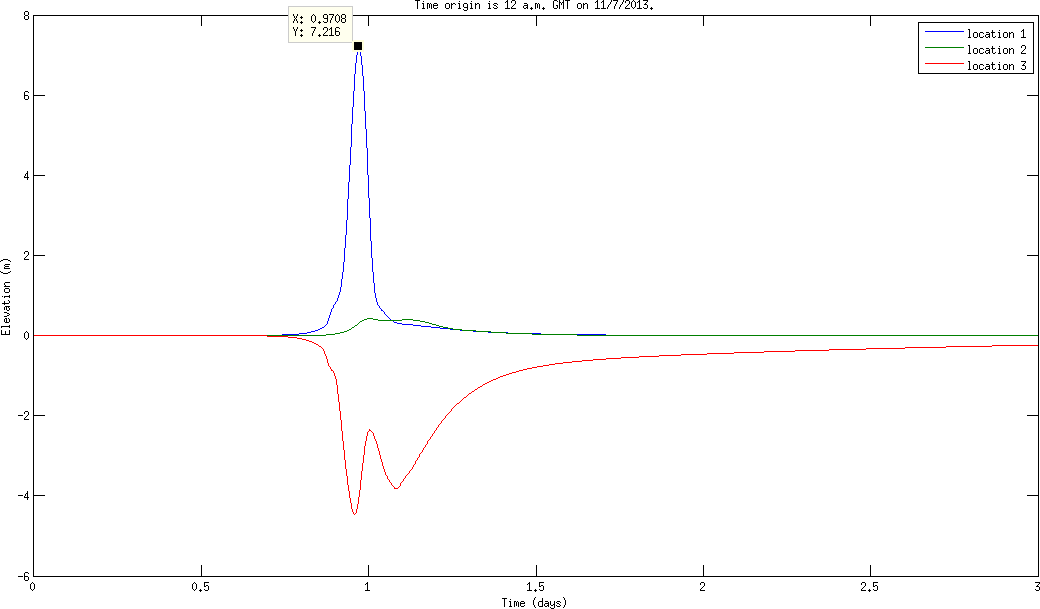
\includegraphics[width=.5\textwidth]{G/g0-001}
		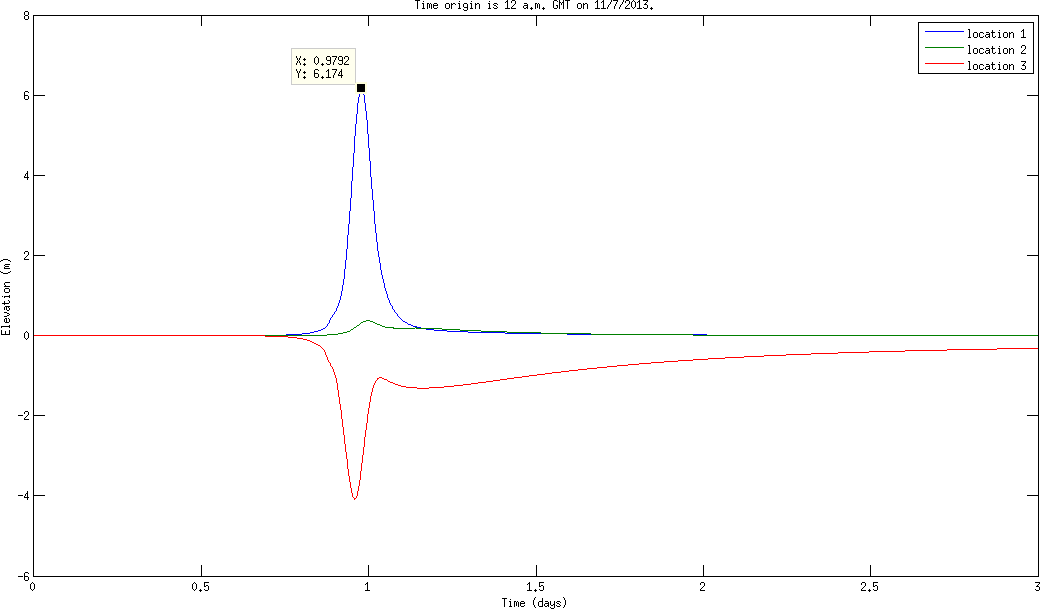
\includegraphics[width=.5\textwidth]{G/g0-005}
		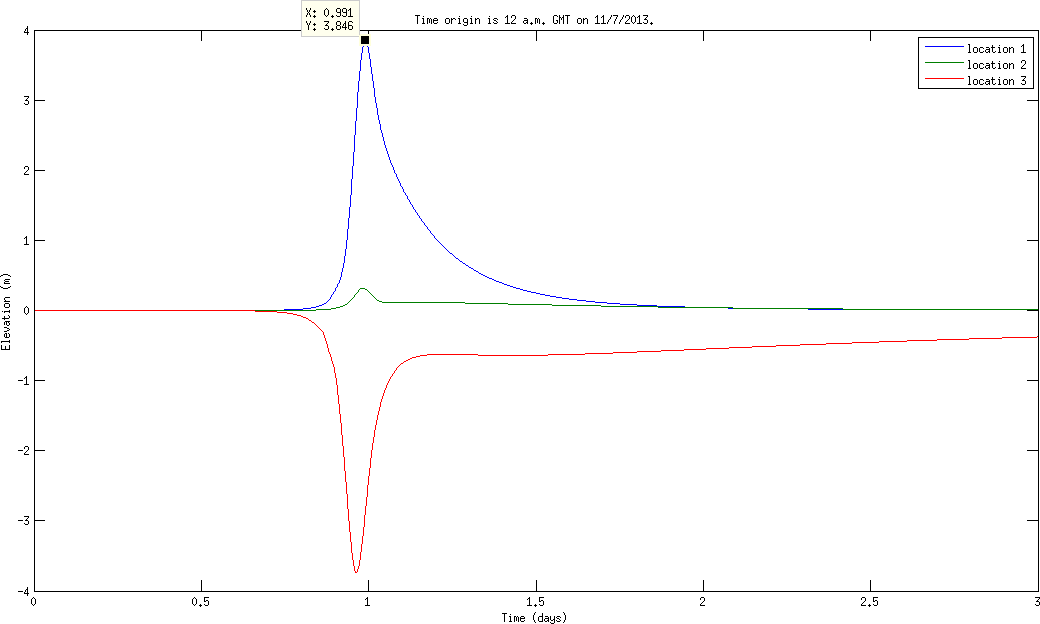
\includegraphics[width=.5\textwidth]{G/g0-05}
		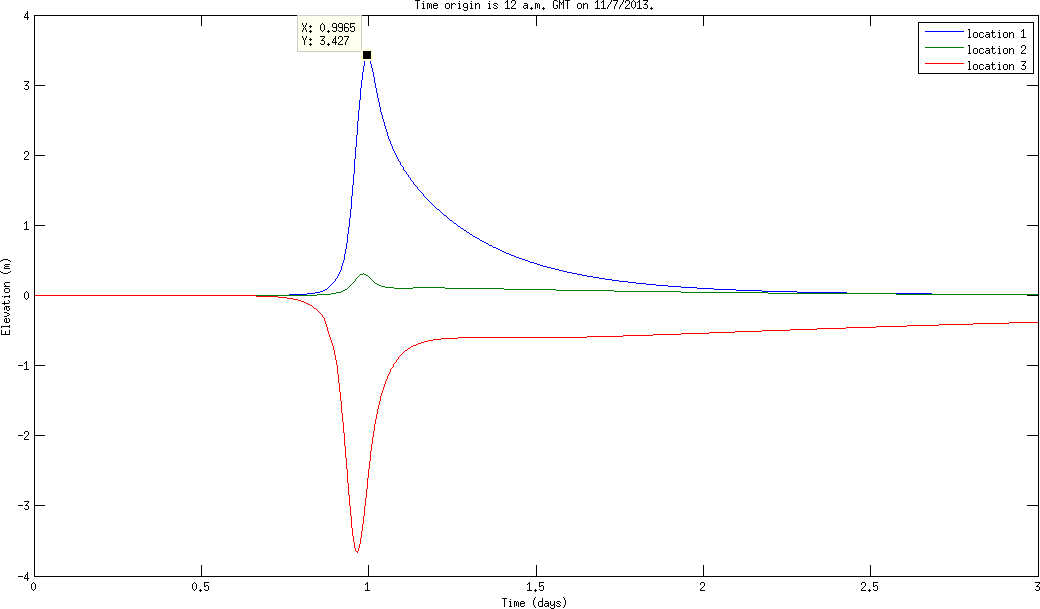
\includegraphics[width=.5\textwidth]{G/g0-10}
	\end{figure}
	\begin{figure}[H]
		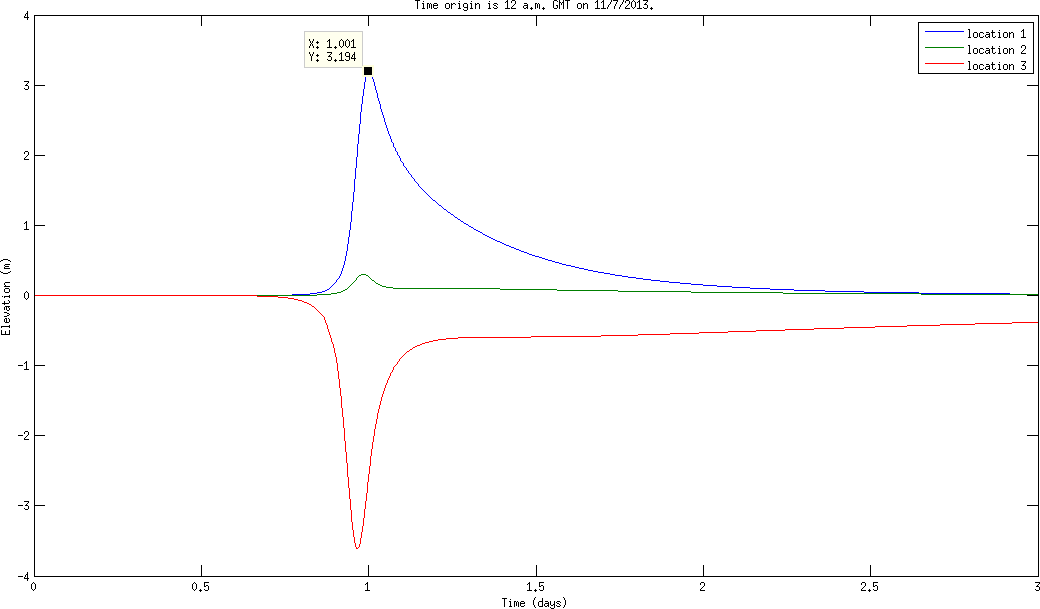
\includegraphics[width=.5\textwidth]{G/g0-15}
		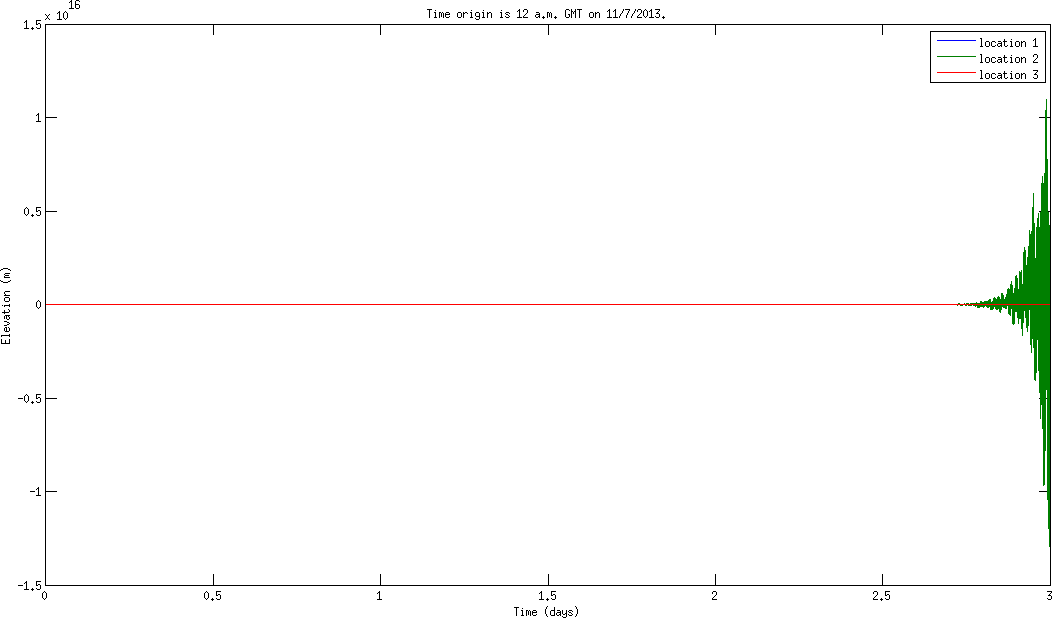
\includegraphics[width=.5\textwidth]{G/g0-20}
	\end{figure}
	
	As $G$ becomes higher, the model becomes unstable and produces oscillations. For lower $G$, we have higher surge height and surge recedes slower than normal.
	
	\section{Conclusion}
	Both our results in storm surge prediction are also similar to the predictions of Project NOAH and Deltares.
	The ADCIRC+SWAN model is chosen to be modified because of its advantages over other models. If we have a more accurate numerical algorithm (together with additive noise), more flexible spatial meshing, and more efficient parallel computation, we can have faster and more realistic real-time predictions.
	
	\begin{thebibliography}{9}
		\bibitem{bib:adcirc}
		R. A. Luettich, Jr., et. al. (1992), \emph{ADCIRC: An Advanced Three-Dimensional Circulation Model, Theory and Methodology}. US Army Engineer Waterways Experiment Station, Vicksburg, Mississippi. \url{http://adcirc.org}
		
		\bibitem{bib:delft}
		Deltares, Delft3D Open Source Community. \url{http://oss.deltares.nl/web/delft3d/home}
		
		\bibitem{bib:app}
		V. P. Bongolan, et. al. (2008), \emph{Stochastic Terms in Boundary Conditions: Applications}. Ellis College of the New York Institute of Technology.
		
		\bibitem{bib:num}
		R. A. Luettich, Jr., et. al. (2004), \emph{Formulation and Numerical implementation of the 2D/3D ADCIRC Finite Element Model Version 44.XX}.
		
		\bibitem{bib:sns}
		F. Flandoli (2013), \emph{State of the art on stochatic Navier-Stokes equations}. Mathematical Paradigms of Climate Science.
		
		\bibitem{bib:wetdry}
		J. C. Dietrich, et. al., \emph{Assessment of ADCIRC's Wetting and Drying Algorithm}. Institute of Marine Sciences, University of North Carolina, 2005.
		
	\end{thebibliography}
	
\end{document}